\documentclass[12pt]{report}
\usepackage{graphicx}
\usepackage{float}
\begin{document}

\title{Lab3: Free Fall}
\author{Faris Hijazi\\
Student ID: 1039438\\
Partner: Omar Jarrad\\
Section: Thursday 12:30-3:20\\
Professor Noor Eltawil}
\maketitle

\section{Purpose and Theory} 
The purpose of this lab is to experimentally calculate the acceleration due to gravity on an object in free fall. and to compare it to the accepted value of $g = 9.8 m/s^2$.\\
\begin{center}
$a = g$ downwards
\end{center}

\begin{center}
$\Delta{}y = h$
\end{center}

\begin{center}
$v_{i} = 0$
\end{center}

\begin{center}
equation 1:
\end{center}

\begin{center}
$v_{f} = v_{i} + a \Delta{}t$
\end{center}

\begin{center}
$\int$
\end{center}

\begin{center}
$\Delta{}y = \frac{1}{2}(v_{f} + v_{i})\Delta{}t$
\end{center}

\begin{center}
$\frac{1}{2}(v_{f} + v_{i})\Delta{}t= v_{i} + \frac{1}{2}a\Delta{}t^2$
\end{center}
\begin{center}
equation 2:
\end{center}

\begin{center}
$\Delta{}y = v_{i} + \frac{1}{2}a\Delta{}t^2$
\end{center}

\begin{center}
$h = \frac{1}{2}gt^{2}$
\end{center}

\section{Experiment Apparatus and Procedure}
The clamp and rod are attached to the table, the steel ball is held in a clamp at the top of the rod. The ball completes an electrical circuit while attached, when the ball drops the circuit is broken and stopwatch begins timing until the steel ball touches the metal plate on the floor to stop the timer. three trial are recorded for each of the 8 different heights heights and the average of the three trials at each height is recorded.


\section{Data}

\begin{figure}[H]
    \centering
    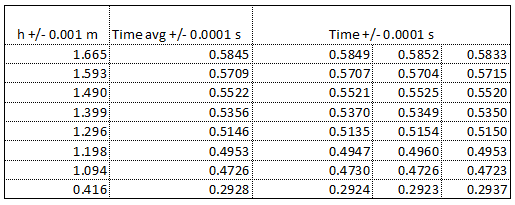
\includegraphics[width=\textwidth]{table}
    \caption{data table}
    \label{fig:table}
\end{figure}

\section{Analysis}

\subsection{Data Analysis}
\begin{figure}[H]
    \centering
    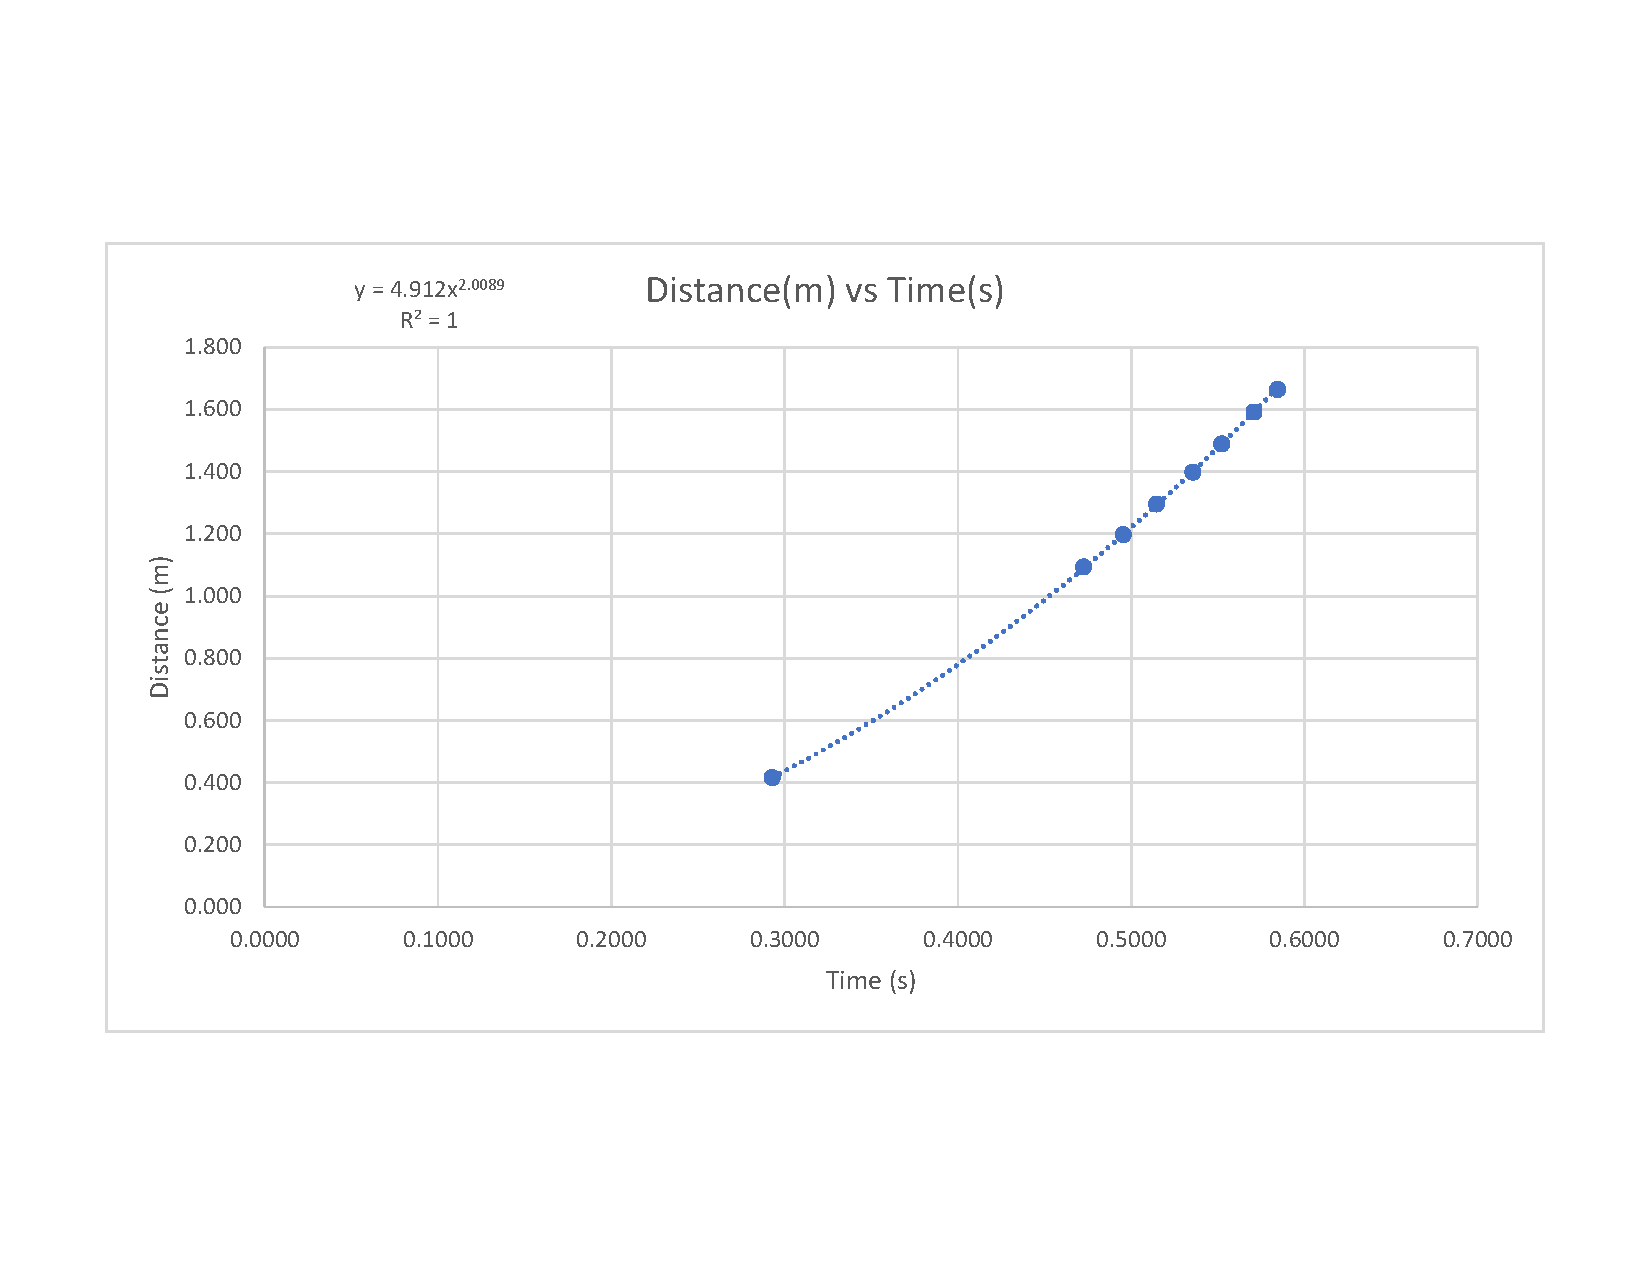
\includegraphics[width=\textwidth]{dvst}
    \caption{distance vs time}
    \label{fig:DvsT}
\end{figure}
\begin{figure}[H]
    \centering
    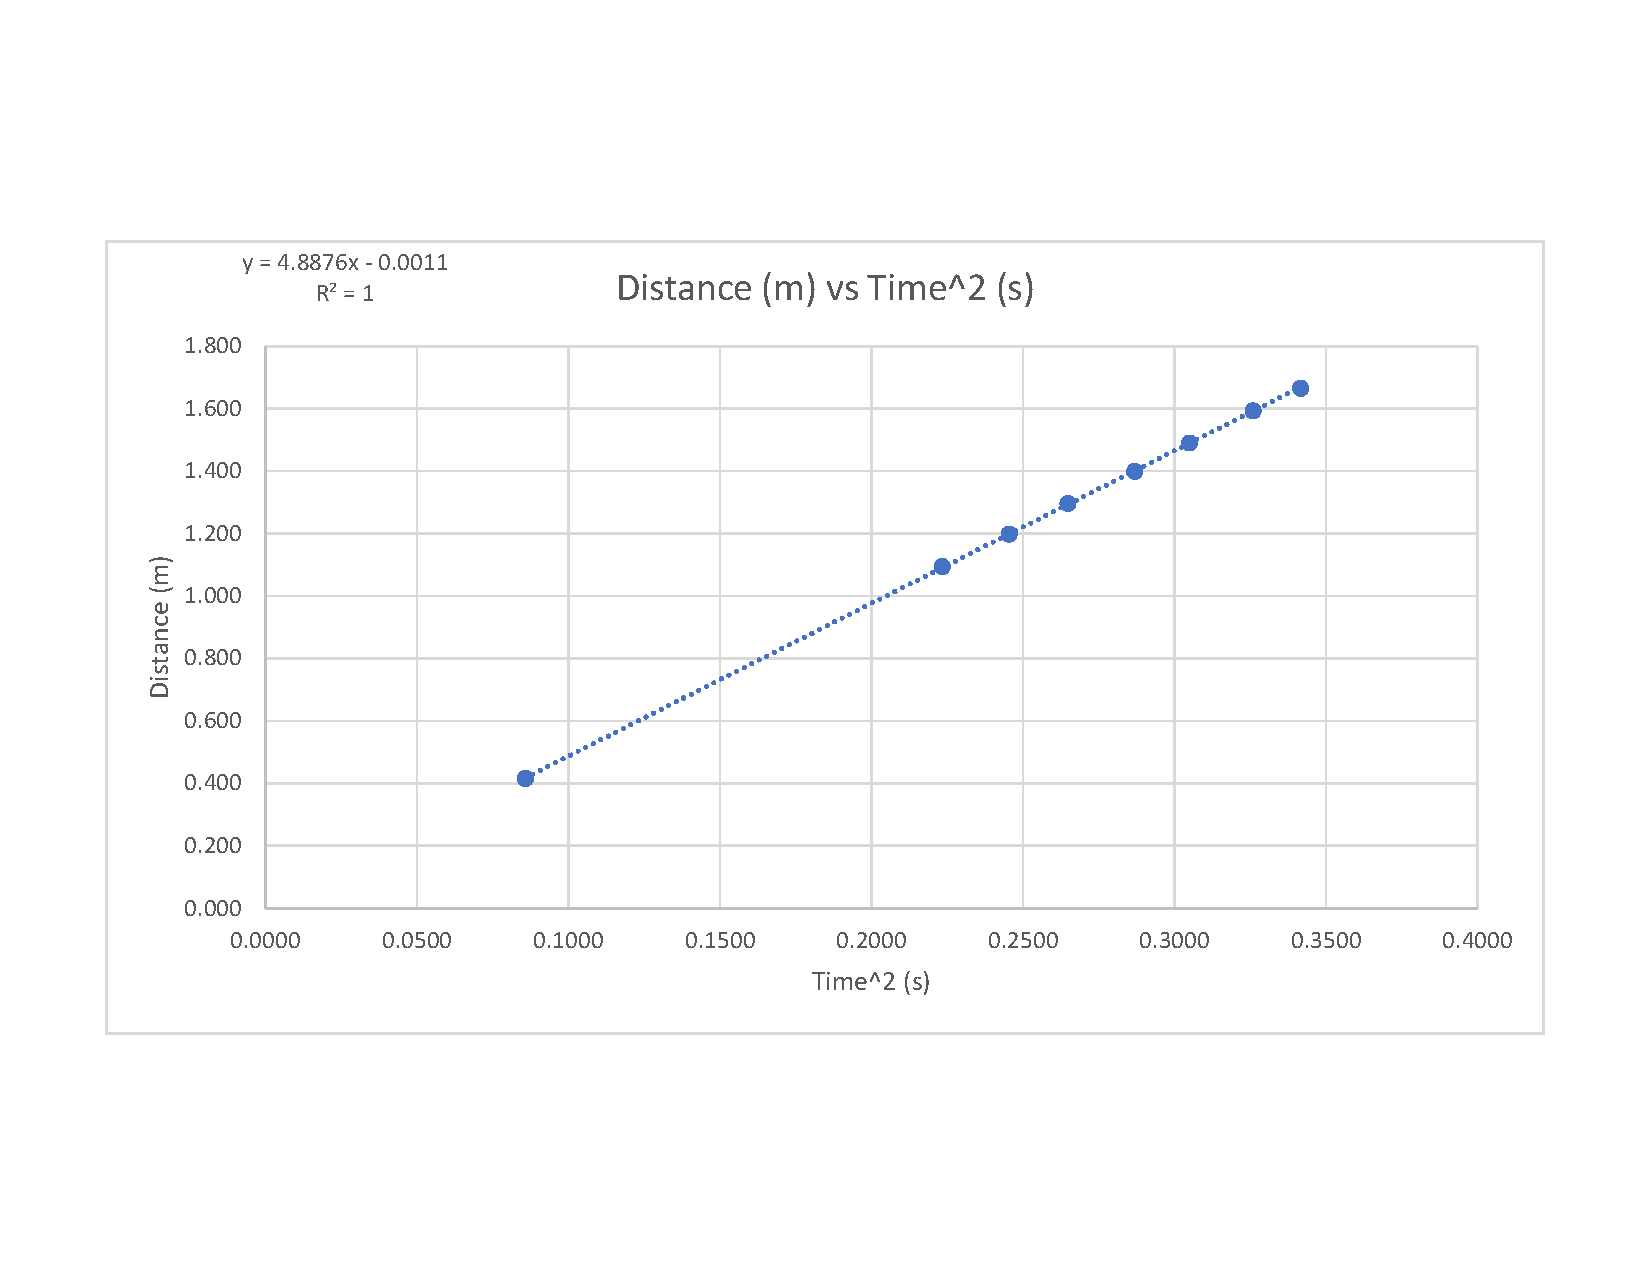
\includegraphics[width=\textwidth]{dvst^2}
    \caption{distance vs $time^{2}$}
    \label{fig:DvsT^2}
\end{figure}
The calculated value of $g = 9.7752 m/s^2$ was achieved by graphing height vs time squared. The slope of this linear trendline is multiplied by 2 to achieve our experimental value for $g$ this is because our derived equation is 
\begin{center}
$h = \frac{1}{2}gt^{2}$
\end{center}
 and thus the linear trend-line as shown in Figure \ref{fig:DvsT^2} has a slope of $\frac{1}{2}g$. $g$ can also be calculated algebraically using the recorded heights and their respective time using the equation $h = \frac{1}{2}gt^{2}$ and solving for $g$, 
\begin{center}
$g = \frac{2h}{t^2}$
\end{center}
\begin{figure}[H]
    \centering
    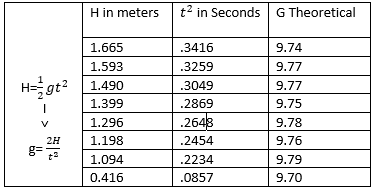
\includegraphics[width=\textwidth]{gravityTable}
    \caption{algebraic $g$}
    \label{fig:gravityTable}
\end{figure}

\subsection{Error Analysis}
The amount of error between the accepted value of $g = 9.8$ $m/s^2$ is very close to the experimental value calculated using the slope of the linear trend-line $g_{exp} = 9.7752$ $m/s^2$
\begin{figure}[H]
\begin{center}
$\mid{} \frac{9.8 m/s^2 -9.7752 m/s^2}{9.8 m/s^2}\mid100$
\label{fig:Percent Error}
\caption{percent error}
\end{center}
\end{figure}

this resulted in a percent error of 0.25\% which is well with the acceptable range.aditionally the standard deviation was found using excel's STDV() function which gave a standard deviation of 0.02633 between each value of $g$ theoretical in Figure \ref{fig:gravityTable} the precision of the instruments was +/- 0.001 m and +/- 0.0001 seconds.
 
\subsection{Results}
\begin{figure}[H]
    \centering
    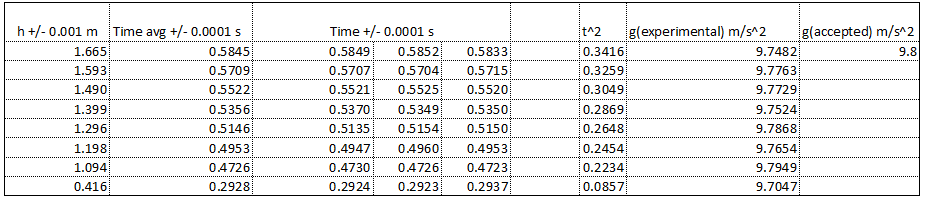
\includegraphics[width=1.25\textwidth]{results}
    \caption{results}
    \label{fig:results}
\end{figure}
\section{Conclusion}
The purpose of this lab was to investigate the affects of free fall and confirm the accepted value of acceleration due to gravity $g = 9.8$ $m/s^2$. This was achieved with an experimental $g_{exp} = 9.7752$ $m/s^2$ with a percent error of only 0.25\% which is well within the margin of error and coincide with the theory.
\end{document}
